% Options for packages loaded elsewhere
\PassOptionsToPackage{unicode}{hyperref}
\PassOptionsToPackage{hyphens}{url}
%
\documentclass[
]{article}
\usepackage{amsmath,amssymb}
\usepackage{lmodern}
\usepackage{iftex}
\ifPDFTeX
  \usepackage[T1]{fontenc}
  \usepackage[utf8]{inputenc}
  \usepackage{textcomp} % provide euro and other symbols
\else % if luatex or xetex
  \usepackage{unicode-math}
  \defaultfontfeatures{Scale=MatchLowercase}
  \defaultfontfeatures[\rmfamily]{Ligatures=TeX,Scale=1}
\fi
% Use upquote if available, for straight quotes in verbatim environments
\IfFileExists{upquote.sty}{\usepackage{upquote}}{}
\IfFileExists{microtype.sty}{% use microtype if available
  \usepackage[]{microtype}
  \UseMicrotypeSet[protrusion]{basicmath} % disable protrusion for tt fonts
}{}
\makeatletter
\@ifundefined{KOMAClassName}{% if non-KOMA class
  \IfFileExists{parskip.sty}{%
    \usepackage{parskip}
  }{% else
    \setlength{\parindent}{0pt}
    \setlength{\parskip}{6pt plus 2pt minus 1pt}}
}{% if KOMA class
  \KOMAoptions{parskip=half}}
\makeatother
\usepackage{xcolor}
\IfFileExists{xurl.sty}{\usepackage{xurl}}{} % add URL line breaks if available
\IfFileExists{bookmark.sty}{\usepackage{bookmark}}{\usepackage{hyperref}}
\hypersetup{
  pdftitle={Untitled},
  hidelinks,
  pdfcreator={LaTeX via pandoc}}
\urlstyle{same} % disable monospaced font for URLs
\usepackage[margin=1in]{geometry}
\usepackage{longtable,booktabs,array}
\usepackage{calc} % for calculating minipage widths
% Correct order of tables after \paragraph or \subparagraph
\usepackage{etoolbox}
\makeatletter
\patchcmd\longtable{\par}{\if@noskipsec\mbox{}\fi\par}{}{}
\makeatother
% Allow footnotes in longtable head/foot
\IfFileExists{footnotehyper.sty}{\usepackage{footnotehyper}}{\usepackage{footnote}}
\makesavenoteenv{longtable}
\usepackage{graphicx}
\makeatletter
\def\maxwidth{\ifdim\Gin@nat@width>\linewidth\linewidth\else\Gin@nat@width\fi}
\def\maxheight{\ifdim\Gin@nat@height>\textheight\textheight\else\Gin@nat@height\fi}
\makeatother
% Scale images if necessary, so that they will not overflow the page
% margins by default, and it is still possible to overwrite the defaults
% using explicit options in \includegraphics[width, height, ...]{}
\setkeys{Gin}{width=\maxwidth,height=\maxheight,keepaspectratio}
% Set default figure placement to htbp
\makeatletter
\def\fps@figure{htbp}
\makeatother
\setlength{\emergencystretch}{3em} % prevent overfull lines
\providecommand{\tightlist}{%
  \setlength{\itemsep}{0pt}\setlength{\parskip}{0pt}}
\setcounter{secnumdepth}{5}
\usepackage{subfig}
\ifLuaTeX
  \usepackage{selnolig}  % disable illegal ligatures
\fi

\title{Untitled}
\author{}
\date{\vspace{-2.5em}2022-06-11}

\begin{document}
\maketitle

{
\setcounter{tocdepth}{2}
\tableofcontents
}
\hypertarget{r-markdown}{%
\subsection{R Markdown}\label{r-markdown}}

\begin{figure}[h]

{\centering \subfloat[A figure\label{fig:mychunk-1}]{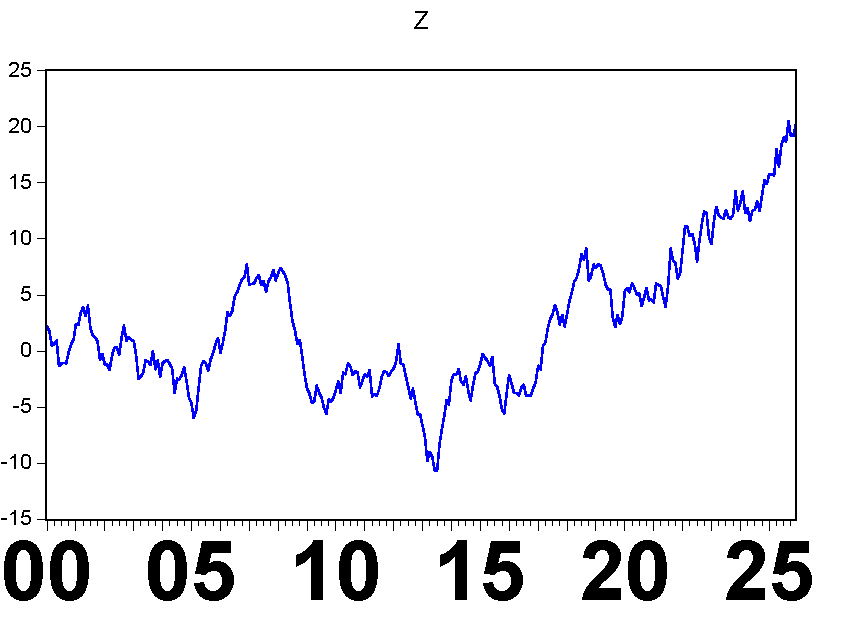
\includegraphics[width=0.5\textwidth]{test_engEviews_files/figure-latex//mychunk-gra2} }\subfloat[Another figure\label{fig:mychunk-2}]{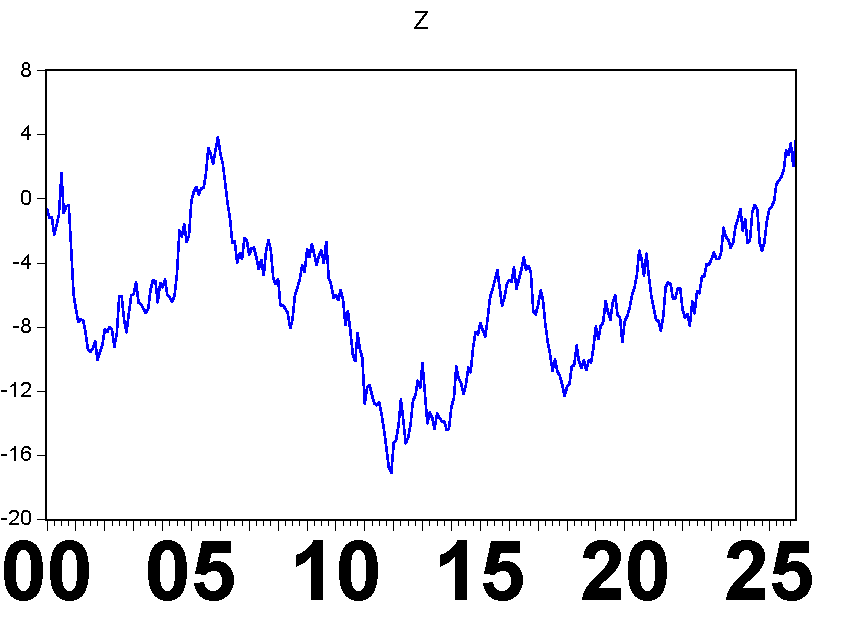
\includegraphics[width=0.5\textwidth]{test_engEviews_files/figure-latex//mychunk-grap1} }\newline\subfloat[A figure\label{fig:mychunk-3}]{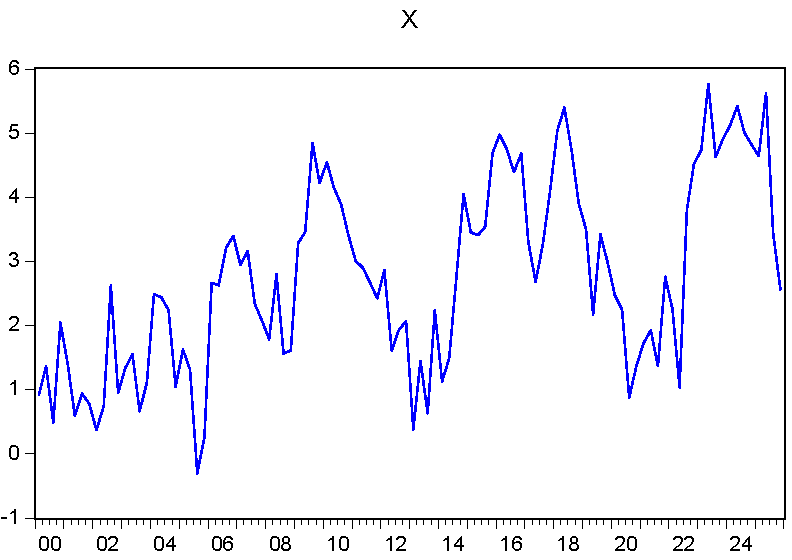
\includegraphics[width=0.5\textwidth]{test_engEviews_files/figure-latex//mychunk-grap} }

}

\caption{somefigure}\label{fig:mychunk}
\end{figure}

holdsagiru

\begin{verbatim}
##        aic  df      coefs       dw        f    fprob       hq      logl
## 1 6.581994 310 -11.273770 0.025327 53.60658 2.12e-12 6.591583 -1024.791
## 2       NA  NA   0.244146       NA       NA       NA       NA        NA
##     meandep ncoef     pval      r2   rbar2 regobs  schwarz    sddep       se
## 1 -15.52534     2 5.28e-44 0.14743 0.14468    312 6.605987 7.007655 6.480926
## 2        NA    NA 2.12e-12      NA      NA     NA       NA       NA       NA
##        ssr  stderrs     tstats
## 1 13020.74 0.686889 -16.412800
## 2       NA 0.033346   7.321651
\end{verbatim}

\hypertarget{r-plots}{%
\section{R plots}\label{r-plots}}

\begin{verbatim}
## [1] "new"
\end{verbatim}

\begin{verbatim}
## [1] "asis"
\end{verbatim}

\begin{center}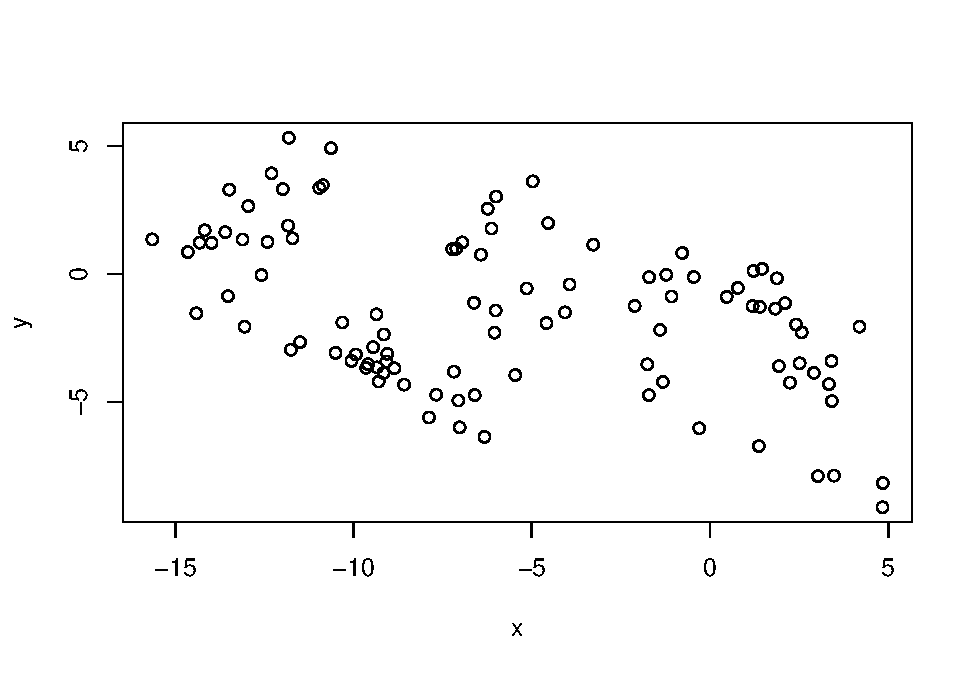
\includegraphics[width=0.5\textwidth]{test_engEviews_files/figure-latex/label-1} \end{center}

\begin{center}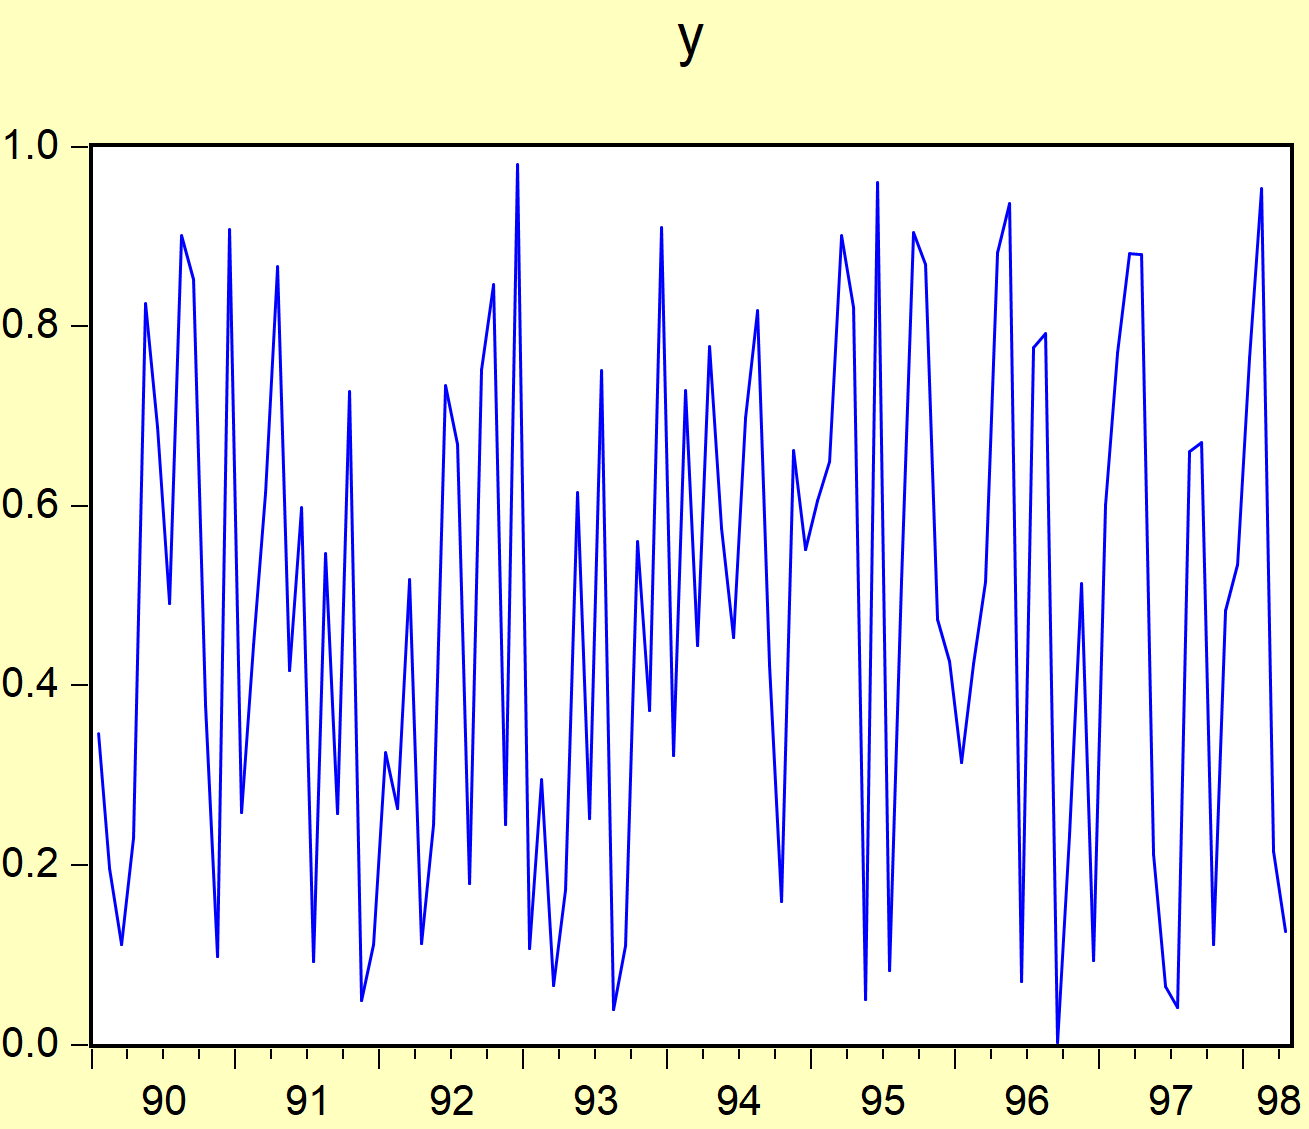
\includegraphics[width=0.5\textwidth]{EViewsR_files/eview-graph-y} \end{center}

\begin{center}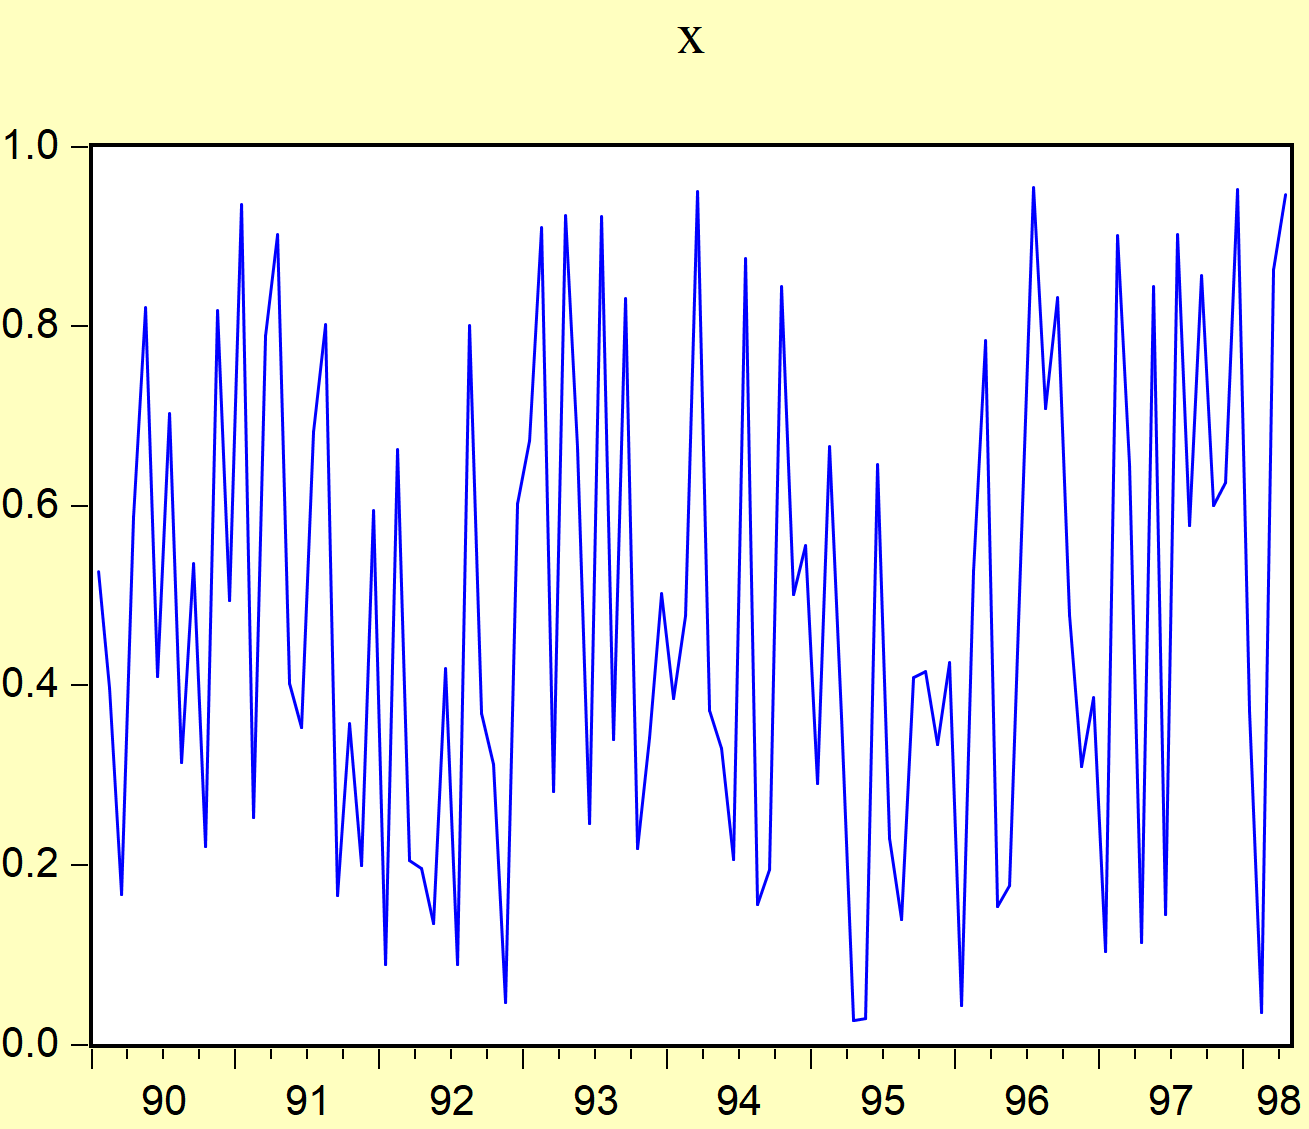
\includegraphics[width=0.5\textwidth]{EViewsR_files/eview-graph-x} \end{center}

\end{document}
